\documentclass[]{article}

\usepackage[T1]{fontenc}
\usepackage[utf8]{inputenc}
\usepackage[french]{babel}
\usepackage[]{graphicx}
\usepackage[]{hyperref}
\usepackage{pdflscape}
\usepackage{tabularx}
\usepackage{float}
\usepackage[table]{xcolor}

\title{Plan de management projet}
\author{
    Responsable\\
    \\
    Julien WATTIER\\
    \\
    \\
    Contributeurs\\
    \\
    Théo DELMAS\\
    Lauric TEYSSEYRE\\
    Pierre-Louis RENON\\
    \\
    \\
    Approbateurs\\
    \\
    Frédéric MIGEON\\
    Gilles LEPINARD\\
    \\
    \\
    Université Paul Sabatier\\
    Master Informatique 1\\
   } 
\date{}


\begin{document}
\maketitle
\newpage
\tableofcontents
\newpage

{
    \setlength{\parindent}{0pt} %Retire les alinéas
    \begin{section}{\label{sec:Objectif du document}Objectif du document}
     Ce document a pour objectif d'exposer les méthodes de management appliquées à ce projet.

     Il permet également de suivre le statut actuel du projet et référencement différents documents de suivi.
    \end{section}

    \begin{section}{\label{sec:Contexte et objectifs du projet}Contexte et objectifs du projet}
     \begin{subsection}{\label{sec:Context}Contexte}
         FlopEDT! est une application permettant de créer un emploi du temps satisfaisant une série de contraintes basées sur la programmation linéaire. Cependant la gestion actuelle de ces contraintes est relativement technique et peu documentée.

         De plus les principaux collaborateurs du projet ont initié un découplage entre le back-end et le front-end, les deux parties étant actuellement gérées par un unique serveur.
     \end{subsection}

     \begin{subsection}{\label{sec:Objectifs}Objectifs}
         L’objectif est de créer un système permettant de récupérer et d’afficher les documentations relatives à des contraintes, le tout respectant le contexte de découplage front/back de l'application.

         Ces demandes sont à l’initiative du principal développeur du projet Pablo SEBAN. Ce projet est donc à façon pour cette même personne.
     \end{subsection}

     \begin{subsection}{\label{sec:Liste des parties prenantes}Liste des parties prenantes}
         Les parties prenantes sont listées ci-dessous ainsi que leurs besoins principaux, leurs représentants, la modalité de validation des besoins et la recette.

         Les utilisateurs finaux et contributeurs seront considérés uniquement au travers du client.

         \begin{subsubsection}{\label{sec:Maître d’ouvrage}Maître d’ouvrage}
             Besoin : Obtenir une interface intuitive pour son produit permettant aux usagers finaux non techniciens de facilement trouver et ajouter des contraintes.

             Représentant : Pablo Seban.

             Validation : voir la \hyperref[sec:Définition de done]{définition de done}.

             Recette : voir la \hyperref[sec:Gestion des besoins]{gestion des besoins}.
         \end{subsubsection}

         \begin{subsubsection}{\label{sec:Collaborateur du projet}Collaborateur du projet}
             Besoin : Obtenir une nouvelle version du système maintenable.

             Représentant : Pablo Seban.

             Validation : voir la \hyperref[sec:Définition de done]{définition de done}.

             Recette : voir la \hyperref[sec:Gestion des besoins]{gestion des besoins}.
         \end{subsubsection}

         \begin{subsubsection}{\label{sec:Utilisateur final}Utilisateur final}
             Besoin : Obtenir une nouvelle version du système utilisable avec efficacité.

             Représentant : Pablo Seban.

             Validation : voir la \hyperref[sec:Définition de done]{définition de done}.

             Recette : voir la \hyperref[sec:Gestion des besoins]{gestion des besoins}.
         \end{subsubsection}

         \begin{subsubsection}{\label{sec:Fournisseur}Fournisseur}
             Besoin : Satisfaire au mieux les demandes du client.
             Monter en compétence.

             Représentants : Théo DELMAS, Lauric TEYSSEYRE, Pierre-Louis RENON, Julien WATTIER.

             Validation : Non concernée.

             Recette : Non concernée.
         \end{subsubsection}

         \begin{subsubsection}{\label{sec:Assistant de maîtrise d’ouvrage}Assistant de maîtrise d’ouvrage}
             Besoin : Répondre aux demandes de soutien de la part du maître d'ouvrage dans la gestion de ce projet.

             Représentants : Léo CUSSEAU, Florian AZIZEN.

             Validation : Non concernée.

             Recette : Non concernée.
         \end{subsubsection}

         \begin{subsubsection}{\label{sec:Professeur}Professeur}
             Besoin : Obtenir des documents de gestion clairs et de qualité.

             Représentants : Frédéric MIGEON, Gilles LEPINARD.

             Validation : Défini lors des cours relatifs à l’UE.

             Recette : Évaluation itérative des documents tous les mois.
         \end{subsubsection}
     \end{subsection}
    \end{section}

    \newpage

    \begin{section}{\label{sec:Référentiel de management de projet}Référentiel de management de projet}
     \begin{subsection}{\label{sec:Product Breakdown Structure}Product Breakdown Structure}
         Le product breakdown structure défini l’ensemble des produits que doit produire ce projet. Pour chaque produit la méthode de réalisation est présentée.

         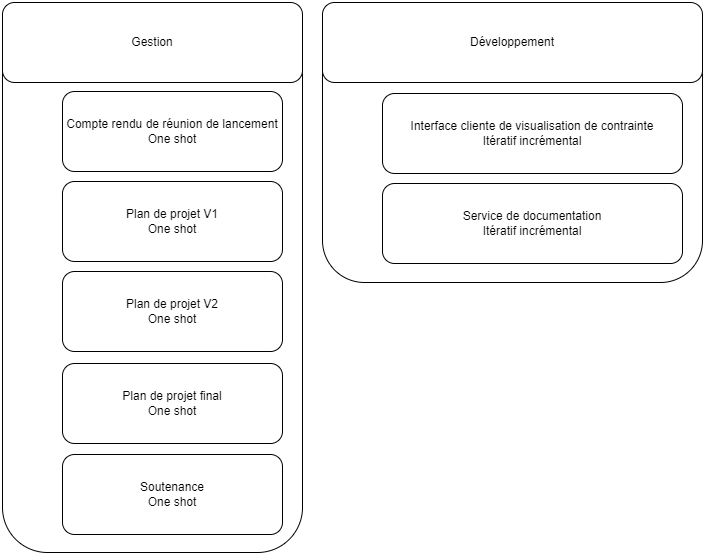
\includegraphics[scale=0.4]{documents/IMG/PBS}
     \end{subsection} 

     \newpage

     \begin{subsection}{\label{sec:Activités du projet}Activités du projet}
         \begin{subsubsection}{\label{sec:Work Breakdown Structure}Work Breakdown Structure}
             Le work breakdown structure défini l’ensemble des activités nécessaires pour réaliser ce projet. Il s’organise en deux parties : La première présente les activités relatives au plan de projet, et la seconde celles au développement, découpées en sprint.

             Ces deux grandes parties sont effectuées en parallèle. Cependant le contenu de ces parties est effectué de manière séquentielle à cause de leur dépendance. Chaque nœud de la structure précise quelles sont ses entrées et ses sorties.

             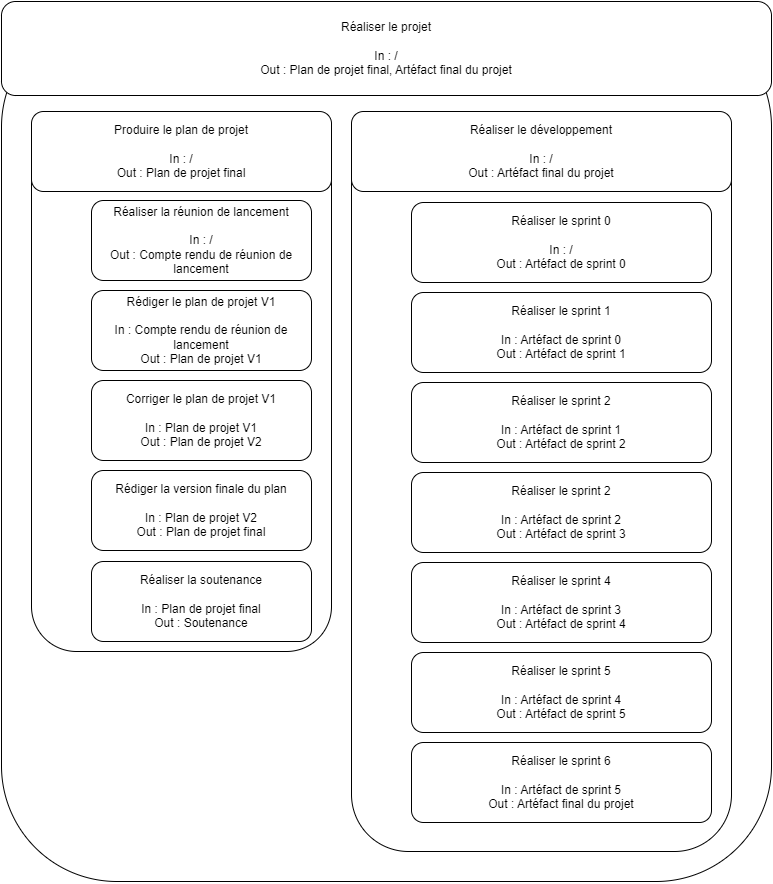
\includegraphics[scale=0.45]{documents/IMG/WBS}
         \end{subsubsection}

         \newpage

         \begin{subsubsection}{\label{sec:Calendrier des ressources}Calendrier des ressources}
             Ce projet est sans ressource matérielle.

             Concernant l’équipe, elle est disponible le jeudi et le vendredi sur la période fixe du 05/01/2023 au 28/04/2023. Les horaires restent souples mais chaque membre est disponible au moins 7 heures sur ces deux jours.

             L’équipe est en congé le 02/03/2023 et le 03/03/2023.
         \end{subsubsection}

         \begin{subsubsection}{\label{sec:Liste des jalons}Liste des jalons}
             L’équipe effectue des sprints de deux semaines.

             Le premier sprint est cependant plus long afin de préparer l’environnement du projet.

             Les différents jalons liés au développement sont les suivants :
             \begin{itemize}
                 \item Fin de sprint 0 (03/02/2023)
                 \item Fin de sprint 1 (17/02/2023)
                 \item Fin de sprint 2 (10/03/2023)
                 \item Fin de sprint 3 (24/03/2023)
                 \item Fin de sprint 4 (07/04/2023)
                 \item Fin de sprint 5 (21/04/2023)
                 \item Fin de sprint 6 (28/04/2023)
             \end{itemize}

             Concernant la partie management, les jalons sont relatifs aux dates de rendu du plan projet. Ils sont donc les suivants :
             \begin{itemize}
                 \item 17/02/2023 : premier rendu intermédiaire du plan projet.
                 \item 17/03/2023 : second rendu intermédiaire du plan projet.
                 \item 14/04/2023 : rendu final du plan projet.
             \end{itemize}
         \end{subsubsection}

         \begin{subsubsection}{\label{sec:Prévision de la charge de travail}Prévision de la charge de travail}
             Le haut degré d’inconnu dans ce projet fait qu’aucune prévision de travail (Gantt) n’est établie car risquant d’être trop éloignée de la réalité.

             Pour ce qui concerne les tâches plus « atomiques », faute d’expérience dans le développement et dans la gestion, l’équipe n’applique pas de prévision de la charge de travail car cette dernière serait certainement erronée et ferait perdre du temps à l’équipe.
         \end{subsubsection}
     \end{subsection}

\newpage

     \begin{subsection}{\label{sec:Rôles et responsabilités}Rôles et responsabilités}
         \begin{subsubsection}{\label{sec:Organizational Breakdown Structure}Organizational Breakdown Structure}
             Le schéma ci-dessous présente une hiérarchie des différents rôles de ce projet, leurs représentants ainsi qu’une description de chacun.

             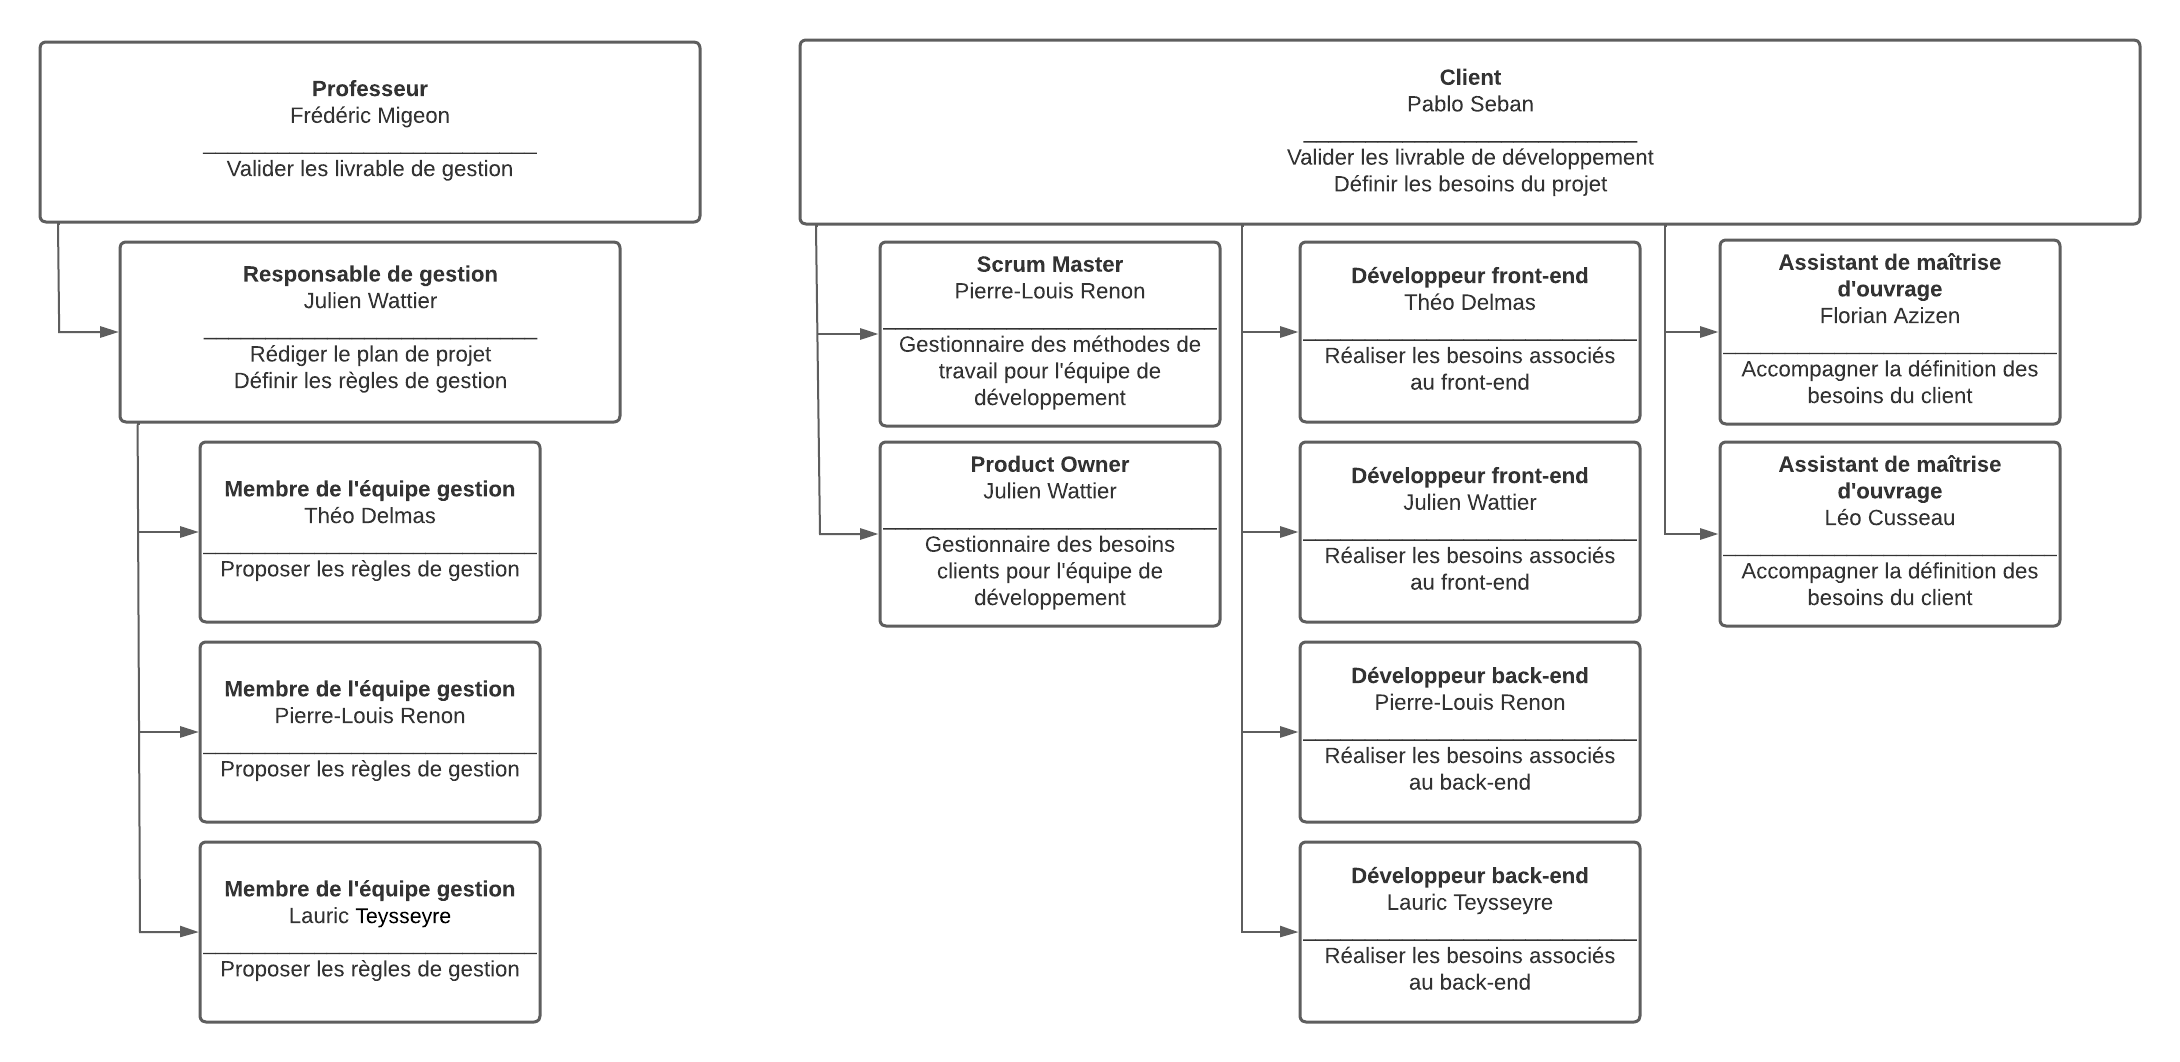
\includegraphics[scale=0.32]{documents/IMG/OBS}
         \end{subsubsection}

         \begin{subsubsection}{\label{sec:Matrice RACI}Matrice RACI}
             La matrice suivante définit les responsabilités de chaque activité pour chaque rôle. Cette responsabilité est définie selon la codification suivante :
             \begin{itemize}
                 \item[R]: Est responsable de la tâche.
                 \item[A] : Valide ou non la tâche lorsqu’elle est réalisée.
                 \item[C] : Contribue à la réalisation de la tâche.
                 \item[I] : Est informé des avancements et décisions relatives à la tâche.
             \end{itemize}

             \begin{landscape}
                \begin{table}[H]
                    \caption{Matrice RACI}
                    \fontsize{8pt}{9pt}\selectfont
                    \begin{tabularx}{\columnwidth}{|X|X|X|X|X|X|X|X|X|X|}
                        \hline
                        & Professeur & Responsable de gestion & Membre de l'équipe de gestion & Client & Scrum Master & Product owner & Développeur front-end & Développeur back-end & AMO\\
                        \hline
                        Réaliser la réunion de lancement & A & R & C & C &  &  &  &  & \\
                        \hline
                        Rédiger le plan V1& A & R & C &  &  &  &  &  & \\
                        \hline
                        Corriger le plan V1& A & R & C &  &  &  &  &  & \\
                        \hline
                        Corriger le plan V2& A & R & C  &  &  &  &  &  & \\
                        \hline
                        Rédiger la version finale du plan& A & R & C  &  &  &  &  &  & \\
                        \hline
                        Réaliser la soutenance& A & R & C  &  &  &  &  &  & \\
                        \hline
                        Réaliser le sprint 0&  &  &  & A & R & R & C & C & I\\
                        \hline
                        Réaliser le sprint 1&  &  &  & A & R & R & C & C & I\\
                        \hline
                        Réaliser le sprint 2&  &  &  & A & R & R & C & C & I\\
                        \hline
                        Réaliser le sprint 3&  &  &  & A & R & R & C & C & I\\
                        \hline
                        Réaliser le sprint 4&  &  &  & A & R & R & C & C & I\\
                        \hline
                        Réaliser le sprint 5&  &  &  & A & R & R & C & C & I\\
                        \hline
                        Réaliser le sprint 6&  &  &  & A & R & R & C & C & I\\
                        \hline
                    \end{tabularx}
                \end{table}
             \end{landscape}
         \end{subsubsection}
     \end{subsection}

     \begin{subsection}{\label{sec:Suivi de déroulement}Suivi de déroulement}
         \begin{subsubsection}{\label{sec:Suivi du contexte}Suivi du contexte}
             Les événements s'étant produits durant le projet sont référencés dans le \href{documents/Registre_des_faits_marquants.pdf}{registre des faits marquants}. Ces événements sont regroupés par sprint et catégorisés comme étant positif ou négatif.
         \end{subsubsection}

         \begin{subsubsection}{\label{sec:Gestion des décision}Gestion des décision}
             Les décisions relatives au projet sont traçables dans le \href{documents/Registre_des_décisions.pdf}{registre des décisions}.

             Chaque décision y est décrite par sa description, qui précise ce qu’elle a modifié dans le plan projet, la justification/le contexte ayant nécessité cette décision ainsi que la date.

             Lorsqu’une décision est créée, le plan projet est alors actualisé conformément à la décision et mis à jour par ajout d'un sur l’outil de gestion de version associé (voir la \hyperref[sec:Communication avec les parties prenantes]{communication avec les parties prenantes}).
         \end{subsubsection}

         \begin{subsubsection}{\label{sec:Gestion des actions}Gestion des actions}
             Le suivi des actions à réaliser/réalisé est disponible sur le kanban grâce aux listes de tâches qu’il est possible d’associer à un besoin(voir \hyperref[sec:Référencement des besoins]{le référencement des besoins}).
         \end{subsubsection}
     \end{subsection}

     \begin{subsection}{\label{sec:Gestion de la communication}Gestion de la communication}
         \begin{subsubsection}{\label{sec:Communication avec les parties prenantes}Communication avec les parties prenantes}
             Les communications avec les professeurs sont faites de manière informelle lors de TD dédié à l’UE de projet.

             Pour les communications avec le client, elles se font au travers du discord de FlOpEDT, que ce soit de manière textuelle pour des questions spontanées, ou vocale pour ce qui concerne les revues de sprint. Ces dernières se tenant dans les jours suivant la fin d’un sprint, fonction des disponibilités de chacun.

             Les revues de sprint sont enregistrées, puis traitées ultérieurement afin de produire un compte rendu de réunion référencé dans le \href{documents/Registre_des_rapports_de_réunion.pdf}{registre des rapports de réunion}. Ces rapports résument les retours du client afin que ces derniers soient référencés en tant qu’action ou décision à réaliser.

             Le reste des parties prenantes n'est pas informé de l’avancée du projet, mais peut le suivre via \href{https://github.com/Szyckaa/UE-PROJET-DOCS-GESTION}{ce dépôt distant} qui trace le plan de projet et les documents liés.
         \end{subsubsection}

         \newpage

         \begin{subsubsection}{\label{sec:Communication au sein de l'équipe}Communication au sein de l'équipe}
             L’équipe communique au travers d’un serveur discord dédié de manière informelle.

             Au début de chaque journée, une daily meeting est organisée pour résumer le travail effectué par chacun lors de la dernière journée, les difficultés rencontrées et le travail prévu sur la journée.

             Le reste de la journée de travail les membres sont tous présents en vocal sur ce même serveur, et partage éventuellement leur écran afin de montrer ce qu’ils font.

             Enfin, pour faciliter le débogage, l’outil de peer-programming liveshare est utilisé.
         \end{subsubsection}
     \end{subsection}

     \begin{subsection}{\label{sec:Gestion de la qualité de management}Gestion de la qualité de management}
         \begin{subsubsection}{\label{sec:Qualité des produits}Qualité des produits}
            L'ensemble des documents est produit en Latex.

            Le plan projet applique le présent descriptif comme style rédactionnel. 

             Les différentes versions du plan de projet sont revues par tous les membres de l’équipe avant soumission en tirant profit des fonctionnalités fournies par l'outil de gestion de version sur lequel ces documents sont suivis (voir la \hyperref[sec:Communication avec les parties prenantes]{gestion de la communication}).

             Chaque version du plan est également soumise à une évaluation interne grâce à une \href{Check_list.ods}{check-list} fournie par les professeurs. Cette liste conserve les réponses des anciennes versions afin d’évaluer l’évolution du plan.

             Enfin, chaque version est revue par les professeurs.
         \end{subsubsection}

         \begin{subsubsection}{\label{sec:Qualité des activités}Qualité des activités}
             L’équipe ne supervise pas les activités de management.
         \end{subsubsection}
     \end{subsection}

     \begin{subsection}{\label{sec:Gestion des risques et opportunités}Gestion des risques et opportunités}
         \begin{subsubsection}{\label{sec:Référencement des risques}Référencement des risques}
             La liste des risques et opportunités est listée dans le \href{documents/Registre_des_risques.pdf}{registre des risques et opportunités}.

             Chaque risque y est décrit par les champs suivants :
             \begin{itemize}
                 \item Titre du risque.
                 \item Description du risque.
                 \item Risque d’occurrence : sur une échelle faible - moyen - fort.
                 \item Niveau d'impact : sur une échelle faible - moyen - fort
                 \item Plan d'action : actions à mettre en place si le risque se déclenche ou est sur le point de se déclencher.
             \end{itemize}

             S'y ajoute les champs suivants à chaque fois qu'il y a déclenchement du risque :
             \begin{itemize}
                 \item Date de déclenchement.
                 \item Contexte de déclenchement.
             \end{itemize}
         \end{subsubsection}

         \begin{subsubsection}{\label{sec:Identification des risques}Identification des risques}
             La majeure partie des risques est identifiée lors de l'élaboration de la note de cadrage.

             Si, lors de la capture d'un besoin, un risque apparaît comme évident aux fournisseurs, il est ajouté dans le registre.
         \end{subsubsection}

         \begin{subsubsection}{\label{sec:Réponse au risques}Réponse au risques}
             En cas de déclenchement d'un risque, l'équipe fournisseur suit le plan d'action prévu dans le registre et remplit les champs associés au déclenchement dans le registre.
         \end{subsubsection}
     \end{subsection}
    \end{section}

\newpage

    \begin{section}{\label{sec:Référentiel de développement de projet}Référentiel de développement de projet}
     L’équipe applique une méthode de développement hybride qui mixe le SCRUM et le kanban. Dans cette méthode, le travail est segmenté temporellement en sprint afin de ne pas perdre de vue le temps. Cependant elle gère les besoins en kanban. Il n’y a donc pas d’estimation de valeur des user stories pour savoir laquelle développer, ni d’objectif de durée pour réaliser un besoin.
     \begin{subsection}{\label{sec:Gestion des besoins}Gestion des besoins}
         \begin{subsubsection}{\label{sec:Référencement des besoins}Référencement des besoins}
             Les besoins sont suivis grâce à ce \href{https://wekan.flopedt.org/b/HsRkBw5rbmQt5PQet/catalogue}{kanban}. Celui-ci se décompose en deux parties. La première définit les principaux produits du projet et permet aux parties prenantes de comprendre sur quel produit l'équipe travaille actuellement. Les produits principaux sont définis lors de la kick-off meeting.

             La seconde est un kanban lié au produit en cours. L'ensemble des besoins y sont retranscrits et décrits grâce à des user stories sur lesquelles l'équipe fournisseur adjoint une liste d'actions à effectuer afin de satisfaire la user story.

             Le kanban se divise en 5 colonnes :
             \begin{itemize}
                 \item Idée floue : La user story nécessite d'être raffinée en ajoutant les actions à effectuer qui y sont relatives. Cette colonne permet de noter informellement les besoins du client.
                 \item À faire : La user story est définie mais pas choisie pour le sprint en cours.
                 \item En cours : La user story est choisie pour le sprint en cours.
                 \item À tester : La user story est satisfaite mais nécessite une validation via des tests unitaires et d’intégration, une approbation de la part du client, ainsi qu’une documentation du code source.
                 \item Ok : La user story valide la définition de done et est livrée à la fin du sprint courant.
             \end{itemize}

             Chaque user story est priorisée via sa position dans son couloir.

             Cet outil mixe donc le backlog ; puisqu’il référence les besoins ; et le kanban ; puisque les tâches à effectuer sont ajoutées au sein de chaque besoin.

             Chaque développeur peut manipuler le kanban sans autorisation particulière.
         \end{subsubsection}

         \begin{subsubsection}{\label{sec:Définition de ready}Définition de ready}
            L'ensemble des critères suivants représentent la définition de ready des besoins traités ; c'est-à-dire que le besoin est passé en "A faire" (voir \hyperref[sec:Référencement des besoins]{référencement des besoins}) : 
            \begin{itemize}
                \item Le besoin est décrit par une user story sous la forme "En tant <catégorie d'utilisateurs> je désire <fonctionnalité> afin de <intérêt de la fonctionnalité>.
                \item Une première liste d'actions nécessaires pour réaliser ce besoin a été adjointe au besoin.
                \item Chaque développeur a approuvé la description textuelle et la liste d'actions à effectuer.
            \end{itemize}
        \end{subsubsection}

        \begin{subsubsection}{\label{sec:Définition de done}Définition de done}
            L'ensemble des critères suivants représentent la définition de done des besoins traités ; c'est-à-dire que le besoin est passé en "OK" (voir \hyperref[sec:Référencement des besoins]{référencement des besoins}) : 
            \begin{itemize}
                \item Le développement relatif au besoin est terminé.
                \item Les règles de qualité développement sont respectées(voir la \hyperref[sec:Gestion de la qualité]{gestion de la qualité})
            \end{itemize}
        \end{subsubsection}

         \begin{subsubsection}{\label{sec:Capture des besoins}Capture des besoins}
             Une première partie des besoins est capturée lors de la kick-off meeting et sa préparation.

             Les besoins sont capturés lors des revues de sprint en fonction des remarques du client sur ce qui est présenté. Lors de la production du rapport de revue (voir la \hyperref[sec:Gestion de la communication]{gestion des communications}) dans les jours suivant la réunion, les besoins sont alors raffinés et placés en "à faire".

             Si un nouveau besoin fait apparaître un nouveau produit, alors une décision sera émise pour faire changer le référentiel.

             Le client définit oralement la nouvelle priorité des besoins à réaliser à chaque sprint.
         \end{subsubsection}

         \begin{subsubsection}{\label{sec:Gestion des changement dans les besoins}Gestion des changement dans les besoins}
             Lors des revues de sprint le client a la possibilité d’émettre des remarques pouvant faire évoluer les besoins et tâches.

             Lors de la production du rapport de revue (voir la \hyperref[sec:Gestion de la communication]{gestion des communications}) dans les jours suivant la réunion, ces remarques sont alors transformées en actions et ajoutées sur le besoin associé.
         \end{subsubsection}
     \end{subsection}

     \begin{subsection}{\label{sec:Gestion du développement}Gestion du développement}
         Le développement suit le workflow git. Il y a donc une branche maîtresse intégrant les releases (artefact d’un sprint), une branche de développement intégrant les features en cours de développement et des branches de features correspondant au traitement d’un besoin.
     \end{subsection}

     \begin{subsection}{\label{sec:Gestion de la configuration}Gestion de la configuration}
         Les produits de ce projet seront tracés à l'aide de git, sur le \href{https://framagit.org/flopedt/FlOpEDT}{dépôt officiel de FlopEDT}, et en particulier sur la branche \href{https://framagit.org/flopedt/FlOpEDT/-/tree/catalog}{catalog}.

         Chaque développeur dispose des droits et responsabilités sur les actions qu'il entreprend relativement à ce dépôt.
     \end{subsection}

     \begin{subsection}{\label{sec:Gestion des livrables}Gestion des livrables}
         \begin{subsubsection}{\label{sec:Processus de livraison}Processus de livraison}
             Lorsque les fonctionnalités sont considérées comme terminées elles sont intégrées dans la branche maîtresse, ce qui marquera la livraison au client.

             L’équipe s’assurer d’intégrer uniquement des fonctionnalités terminées donc fonctionnelles.
         \end{subsubsection}

         \begin{subsubsection}{\label{sec:Suvi des livraisons}Suvi des livraisons}
             Les commits de merge dans la branche maîtresse depuis la branche de développement (voir la \hyperref[sec:Gestion du développement]{gestion du développement}) permettent de tracer les livrables livrés.
         \end{subsubsection}

         \begin{subsubsection}{\label{sec:Livraison finale}Livraison finale}
             Une revue de code est organisée avec le client et des collaborateurs du projet au moment de la dernière livraison afin de faciliter la reprise du travail produit. La livraison finale est faite selon les modalités classiques (voir le \hyperref[sec:Processus de livraison]{processus de livraison}).
         \end{subsubsection}
     \end{subsection}

     \begin{subsection}{\label{sec:Gestion de la qualité}Gestion de la qualité}
         \begin{subsubsection}{\label{sec:Front-end}Front-end}
             Le code produit est soumis à l’outil de vérification ESLint, ce qui permet d’avoir une syntaxe homogène mais également d’optimiser le code en appliquant des bonnes pratiques qui sont vérifiées par l’outil.

             Le code est documenté en ajoutant de la JSDoc à chaque méthode, variable et classe et en tirant profit des annotations offertes par la JSDoc. Concernant les composants, ils sont documentés à l’aide d’un entête au début de la section de script qui récapitule ce que fait le composant. Après cet entête se trouvent les paramètres du composant, puis les événements émissibles. Ainsi l’ensemble de l’interface du composant est localisé au même endroit et est documenté.
         \end{subsubsection}

         \begin{subsubsection}{\label{sec:Back-end}Back-end}
             L’essentiel des développements back-end consiste à produire des API utilisées par le front-end. Ces API sont développées selon la convention RESTFull.

             Le code est documenté en ajoutant de la documentation à chaque méthode, variable et classe.
         \end{subsubsection}

         \begin{subsubsection}{\label{sec:Revue de code}Revue de code}
             L’équipe tire profit des fonctionnalités de l’outil de gestion de version (voir la \hyperref[sec:Gestion de la configuration]{gestion de la configuration}) en imposant une revue de code avant d’intégrer une fonctionnalité dans la branche de développement. L’intégration doit être validée par au moins deux développeurs différents de celui qui a développé la fonctionnalité.
         \end{subsubsection}

         \begin{subsubsection}{\label{sec:Revue de sprint}Revue de sprint}
             Les revues de sprint permettent la validation orale du client sur un besoin, afin de savoir si la réalisation de ce dernier par l’équipe de développement correspond bien à ses attentes.
         \end{subsubsection}
     \end{subsection}
    \end{section}

    \begin{section}{\label{sec:Bilan de projet}Bilan de projet}
     \begin{subsection}{\label{sec:Référencement du bilan}}
         Le bilan est référencé dans le \href{documents/Bilan_de_projet.pdf}{document dédié}.
     \end{subsection}

     \begin{subsection}{\label{sec:Production du bilan}}
         Le bilan est produit après livraison de la dernière version du plan projet durant la semaine du 24/04/2023.
         Ce dernier, ainsi que le documents évolutifs mis à jour relativement aux derniers événemenst du projet sont disponibles au travers d’une release sur l’outil de gestion de version qui trace les documents de gestion (voir la \hyperref[sec:Communication avec les parties prenantes]{communication avec les parties prenantes}).
     \end{subsection}
    \end{section}
}

\end{document}